\documentclass[11pt]{article}

% Change "review" to "final" to generate the final (sometimes called camera-ready) version.
% Change to "preprint" to generate a non-anonymous version with page numbers.
\usepackage[preprint]{acl}

% Standard package includes
\usepackage{times}
\usepackage{latexsym}
\usepackage{amsmath}
\usepackage{tikz}
\usetikzlibrary{shapes.geometric, arrows, positioning, arrows.meta}
\usepackage[T1]{fontenc}
\usepackage[utf8]{inputenc}
\usepackage{microtype}
\usepackage{inconsolata}
\usepackage{graphicx}
\usepackage{xurl}
\usepackage{hyperref}

% figure 1 
\tikzstyle{startstop} = [rectangle, rounded corners, 
minimum width=3cm, 
minimum height=1cm,
text centered, 
draw=black, 
fill=red!30]

\tikzstyle{io} = [ellipse, 
minimum width=3cm,
minimum height=1cm,
align=center,
draw=black,
fill=blue!30
]

\tikzstyle{stack} = [rectangle,
draw=black,
fill=green!30,
align=center,
minimum width=3.2cm,
minimum height=1cm]

\tikzstyle{vector} = [rectangle, rounded corners, 
draw=black,
fill=yellow!30,
align=center, 
minimum width=3.25cm,
minimum height=1cm]

\tikzstyle{ffn} = [rectangle,
draw=black, 
fill=pink!90,
align=center, 
minimum width=7cm,
minimum height=0.5cm,
rotate=90]

\tikzstyle{background} = [rectangle, rounded corners, 
draw=black,
fill=yellow!10,
minimum height=7cm, 
minimum width=4cm]

\tikzstyle{class} = [rectangle, rounded corners, 
draw=black, 
minimum width=3cm,
minimum height=1cm]

\title{Liberta: A Hybrid Transformer-Linguistic Model for Machine-generated Text Detection}

\author{Fabian Kobylanskyj, Barı\c{s} \c{S}im\c{s}ek, Jian Sun \and Jiwoo Lee \\Technical University of Munich, Germany}

\begin{document}

\maketitle

\begin{abstract}

With the rapid advancement of Large Language Models (LLMs) capable of generating text highly resembling human writing, 
a critical task is to distinguish between human written and machine-generated text. This paper describes Liberta, our approach to the 
SemEval 2024 Task 8: \emph{Multidomain, Multimodel and Multilingual Machine-Generated Text Detection}. Our method 
focused on combining RoBERTa embeddings with readability and token-probabilistic features on tackling both the mono- and multilingual track of 
Subtask A: Human vs Machine Text Classification. 
On the official test dataset, our system achieved an accuracy of 88.64\% in the monolingual and 79.87\% in the multilingual track. Our results 
demonstrate that a hybrid approach can significantly enhance the performance in machine-generated text detection compared to a system that solely 
relies on a transformer based architectures. 

\end{abstract}

\section{Introduction}
LLMs have a significant influence on our daily tasks across a wide range of domains, from education and research to 
content creation and communication. Since their impact on society is significantly shaping how we live and work, 
the potential risks associated with them are equally substantial. From spreading misinformation \cite{kreps2022all}, gaining 
unfair advantages in exams to plagiarism \cite{wahle2022large}, and a societal risk when it becomes unclear if 
communication or information comes from a human or machine, there are many dangers and potentially malicious use cases 
that make it crucial to develop automated means for detecting machine-generated text.\\
In response, different detection tools have been developed. However, since a great deal of effort is put into developing
and improving LLMs, the detection of machine-generated text turned out to be an ongoing arms race where the rapid 
improvement of LLMs challenges detectors to deliver accurate results. A striking example for this is the OpenAI 
classifier, which was released in 2023 and discontinued shortly after due to a low rate of accuracy \cite{OPAI}.\\
The SemEval 2024 Task 8: \emph{Multidomain, Multimodel and Multilingual Machine-Generated Text Detection} addresses 
this challenge and provides an incentive to find solutions to the detection of machine-generated text across multiple 
generators \cite{wang2024semeval}. In the following we describe Liberta, our solution to the monolingual track of Subtask A: Human vs Machine Text 
Classification, which is a hybrid model that combines RoBERTa embeddings, readability features and token-level 
probabilistic features.
We also present and discuss the adaption of this hybrid model to the multilingual track of Subtask A, which additionally 
to English includes Arabic, German and Italian. During the development of our models we adhered to the same conditions as participating 
teams in the shared task in order to ensure a fair comparison. 
Our results suggest that a hybrid model that combines those three feature sets can significantly improve 
classification performance and yield a more robust approach than relying on a PLM (Pre-trained Language Model) alone. While RoBERTa successfully 
captures semantic nuances of the input text, the engineered features provide complementary information that RoBERTa 
alone misses. 

\begin{figure*}[t]
    \resizebox{\textwidth}{!}{
    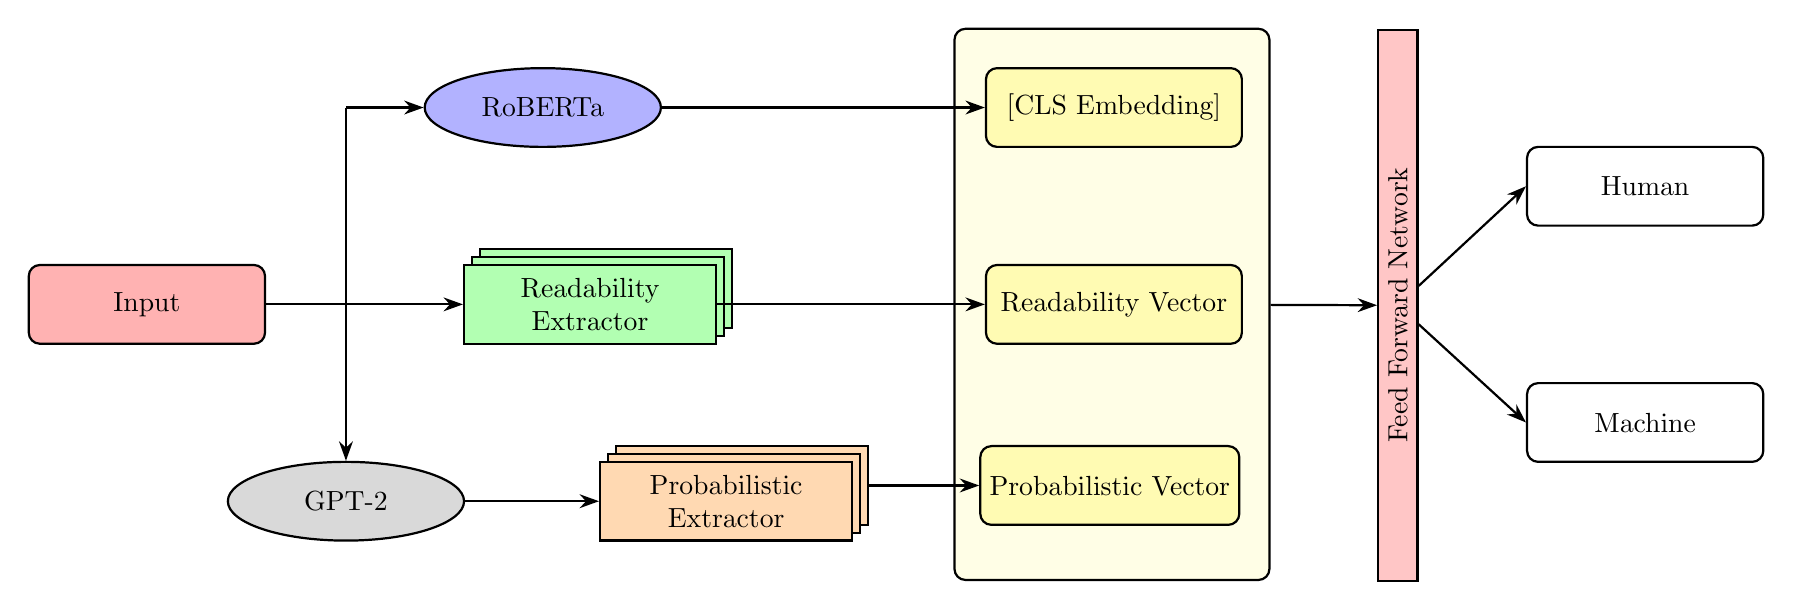
\begin{tikzpicture}[node distance=2cm, thick, 
    >={Stealth[width=5pt,length=7pt]}
    ]
    
    \node (start) [startstop] {Input};
    
    \node (trans) [io, right=of start, yshift=2.5cm] {RoBERTa};
    
    \node (gpt2) [io, right=of start, yshift=-2.5cm, xshift=-2.5cm, fill=gray!30] {GPT-2};
    
    \node (rex2) [stack, right=of start, yshift=0.2cm, xshift=0.7cm] {};
    \node (rex1) [stack, right=of start, yshift=0.1cm, xshift=0.6cm] {};
    \node (rex) [stack, right=of start, xshift=0.5cm] {Readability\\ Extractor};
    
    \node (ex2) [stack, right=of gpt2, yshift=0.2cm, xshift=-0.1cm, fill=orange!30] {};
    \node (ex1) [stack, right=of gpt2, yshift=0.1cm, xshift=-0.2cm, fill=orange!30] {};
    \node (ex) [stack, right=of gpt2, yshift=-0.0cm, xshift=-0.3cm, fill=orange!30] {Probabilistic\\ Extractor};
    
    \node (backvec) [background, right=3.0cm of rex]{};
    
    \node (cls) [vector, right=4.1cm of trans] {[CLS Embedding]};
    \node (rvec) [vector, below= of cls, right=3.4cm of rex] {Readability Vector};
    \node (pvec) [vector, below= of cls, right=1.4cm of ex2] {Probabilistic Vector};
    
    \node (ffn) [ffn, right= of pvec, xshift=-1.225cm] {Feed Forward Network};
    
    \node (human) [class, right= of start, xshift=14cm, yshift=1.5cm] {Human};
    \node (machine) [class, right= of start, xshift=14cm, yshift=-1.5cm] {Machine};
    
    % start arrows
    % split nodes 
    \coordinate (split) at (gpt2|- rex);
    \coordinate (split2) at (gpt2 |-trans);
    
    \draw (start) -- (split);
    \draw (split) edge[->] (gpt2);
    \draw (split) edge[->] (rex);
    \draw (split) -- (split2);
    \draw[->] (split2) -- (trans);
    
    
    \draw (gpt2) edge[->] (ex);
    
    \draw[->] (trans) -- (cls);
    \draw[->] (rex) -- (rvec);
    \draw[->] (ex2) -- (pvec);
    
    \draw[->] (backvec) -- (ffn.north);
    
    \draw[->] (ffn) -- (human.west);
    \draw[->] (ffn) -- (machine.west);
    
    
    \end{tikzpicture}
    }
\caption{Overview of the proposed Hybrid Model Architecture combining three different feature vectors.}
\label{fig:Model}
\end{figure*}

\section{Related Work}
For the binary classification task of machine-generated text detection as in Subtask A, there are two main 
approaches. Zero-shot methods and supervised methods \cite{wang2024semeval}. Zero-shot methods have the advantage of 
not relying on curated datasets of human written and machine-generated text. This can be particularly beneficial in 
the context of the previously mentioned "arms race", where newer LLMs are already far ahead of their predecessors.
Although, zero-shot detectors are considered less accurate, innovations like DetectGPT, which only uses log 
probabilities computed by the model of interest, show that they can accelerate the development of more robust and 
generalizable methods of machine-generated text detection \cite{mitchell2023detectgpt}. \\
In the shared task, however, most prominently used by the participating teams were supervised training methods.
Among those, there are three main groups of methods. The first approach is a fine-tuned detection, which uses a 
pre-trained language model (PLM) and further trains it on the training dataset. Team USTC-BUPT is among the best performing 
teams at the monolingual track of Subtask A only utilizing PLMs. By adding a gradient reversal layer and 
a domain classifier that additionally outputs domain labels they achieved an accuracy of 96.10\% \cite{guo2024ustc}.\\ 
A second major line focuses on statistical and probabilistic methods. These methods build on the principle that LLMs choose tokens
they assign a higher probability to, while humans tend to write in a more "unpredictable" way.
The first ranking Team Genaios employ their model LLMixtic, which mixes token-level probabilistic features from 
four different Llama-2 models forming a feature vector that is fed into a Transformer Encoder. Their method proved 
highly effective, achieving an accuracy of 96.88\% on the monolingual and 75.67\% on the multilingual track \cite{sarvazyan2024genaios}.
Finally, there is a stylometric detection that analyzes linguistic features to distinguish between machine-generated
and human written text. By testing a variety of different features as lexical diversity, text statistics and readability
features and combining them with CLS embeddings from a transformer encoder model, Team PetKaz achieved an accuracy 
of 90.51\% on the monolingual track \cite{petukhova2024petkaz}.


\section{Methodology}

Figure \ref{fig:Model} depicts the architecture of our best performing model. It combines three distinct types of features extracted 
from an input text. The semantic embeddings of a fine-tuned auto-encoder model, different readability metrics and 
token-level probabilistic features. This feature vector is passed through a feed-forward neural network for 
classification. 
\subsection{Semantic Feature Extraction}
We employ RoBERTa-base, fine-tuned on the Machine-generated text classification task. The CLS Token represents the entire 
input sequence and is placed at the beginning of the input, capturing important semantic and contextual information. For 
each input we extract the CLS Token embedding, which for RoBERTa-base is 768-dimensional, and use it as the first part of our 
feature vector. 
\subsection{Readability Feature Extraction}
While today’s LLMs generate grammatically correct and coherent text, their output subtly differs from human written text, 
which we tried to make use of by devoting another part of our feature vector to a detailed linguistic analysis of the 
input sequence. Team Petkaz at the shared task, whose architecture strongly resembles ours, suggests a range of 
linguistic features such as text statistics like the number of difficult words, stylometric features, lexical diversity 
and readability features.\\ 
Based on our data analysis, we decided to include the latter into our model. Previous works suggest that 
machine-generated text tends to be more difficult to read, i.e more complex than human written equivalents. \cite{georgiou2024differentiating} for example, 
reports higher Flesch Reading Ease scores for human texts, which suggest that they are easier to read.
Guided by this thesis, we calculate a variety of readability metrics including the following.\\

\textbf{Flesch Reading Ease and Flesch-Kincaid Grade Level.} Focus on sentence length and syllable count per word.
{\small
\[
    \text{FK} = 0.39 \times \frac{\text{total words}}{\text{total sentences}} + 11.8 \times \frac{\text{total syllables}}{\text{total words}} - 15.59
\]}
The FK Grade-Level was first used by the US army to assess the difficulty of technical manuals. With its weighing factors it 
outputs a U.S. grade level determening the texts difficulty.\\ 

\textbf{Gunning Fog Index.} Asseses sentence complexity by analyzing polysyllabic words.
{\small
\[
    \text{GFI} = 0.4 \times \left(\frac{\text{total words}}{\text{total sentences}} + 100 \times \frac{\text{complex words}}{\text{total words}}\right)
\]}
Words are considered as complex if they consist of three or more syllables. Common suffixes (such as -es, -ed or -ing) are not included. The output is the 
estimated years of education it requires to read a text of this complexity.\\ 

\textbf{Automated Readability Index.} Works like the GFI but instead of counting syllables it counts the number of characters per word and number of words per sentence. 
and outputs a score that maps to a Grade Level from Kindergarten to College Student. 
{\small
\[
    \text{ARI} = 4.71 \times \frac{\text{characters}}{\text{words}} + 0.5 \times \frac{\text{total words}}{\text{total sentences}} - 21.43
\]}

\subsection{Token-Probabilistic Feature Extraction}
Token-probabilistic feature extraction focuses on statistical detection of machine-generated text and follows the core 
hypotheses of machine-generated text being more predictable to LLMs than human-written text. While humans tend to write in a more 
surprising way, LLMs are optimized to choose the next most likely token \cite{holtzman2019curious}. 
To capture these metrics we extract a comprehensive set of features from the token level probability distribution 
generated by GPT-2.\\ 
For a given input text with the tokens \(x_1, x_2,\dots, x_n\), we process the sequence with GPT-2. At the
\(i\)-th position we can extract the probability distribution \(P(x_{i+1} | x_1, \dots, x_i)\) over the entire GPT-2 
Vocabulary. From this distribution we can derive different features. Here, we used features inspired by the work of 
Genaios, the first ranking team in the shared task and got a feature vector including the following metrics, averaged 
across the entire sequence.\\
For each position we calculate (i) the log probability of the observed token, measuring how likely the token is, 
given the tokens already seen. For the feature vector we then use the average observed token probability which 
essentially describes the perplexity of the input sequence. Perplexity is defined as the exponentiated average negative 
log-likelihood of a sequence X with t tokens: 
\[
    ppl(X) = \exp \left( -\frac{1}{t} \sum_{i} \log p_{\theta} (x_i|x_{<i})\right)
\]
Intuitively, it can be thought of as an evaluation of the model’s uncertainty when predicting
the next token. A lower perplexity, and thus a higher average observed 
log-probability, is a strong indicator of machine-generated text. 
We further calculate (ii) the probability of the most likely token, which describes the confidence of the model at each token prediction
step. 
Finally, we take (iii) the entropy, which measures the uncertainty of the distribution. 
\[ \beta_i = - \sum_{y \in \mathcal{V}} p_\theta(y | x_{<i}) \log p_\theta(y | x_{<i})
\] A low entropy would indicate that 
the model is highly confident in a few tokens.  

\subsection{Feed-forward neural network}
The concatenated feature vector is then passed into a feed-forward neural network, where the output layer classifies the text 
as either human or machine-generated text. 

\subsection{Multilingual}
Transferring our previously described system architecture to a multilingual context presented significant challenges. 
Considering that GPT-2 is a transformer model pre-trained on a very large corpus of English data only, the feature 
representation from the token-probabilistic feature extractor was of no use for non-english texts.  
Moreover, readability features are quite language-specific. Applying the same feature for various languages yields very 
inaccurate to irrelevant results. 
To address these challenges, our multilingual approach shifts to a more basic but very effective system relying on a 
fine-tuned XLM-RoBERTa (XLM-R) model. XLM-R is a model trained on 100 different languages, which makes it suitable for 
cross-lingual tasks. Unlike in the monolingual system, we do not apply a self-designed feed-forward neural network, but utilize the transformer library 
that automatically attaches a classification head on top of the model that produces the final classification logits. 

\section{Experiments}
\subsection{Dataset and Evaluation}
We used the SemEval-2024 Task 8 dataset, which is an extension of the M4 dataset \cite{wang2023m4}. 
The training set includes texts from five different domains: Wikipedia, WikiHow, Reddit, arXiv and PeerRead. Machine-generated 
texts were produced by various LLMs, including davinci-003, ChatGPT, Cohere and Dolly-v2. For the test set 
Outfox was used as a surprising domain and GPT-4 and BLOOMz are introduced as surprising generators. The 
labels are roughly balanced with 56,400 machine-generated and 63,351 human-written texts.  
The multilingual training set additionally contains texts in Chinese, Urdu, Bulgarian and Indonesian, and 
for the multilingual test set, Arabic, German and Italian are introduced as unseen languages. 
Table \ref{tab:Dataset} depicts the dataset statistics. 
As in the official shared task setting, we adhered to the rules of not using additional training data. Following the official task description, we used accuracy as the 
evaluation metric to determine the quality of our model.
\begin{table}[ht]
    \centering
    \begin{tabular}{|l|c|c|c|}
    \hline
    \textbf{Track} & \textbf{\#Train} & \textbf{\#Dev} & \textbf{\#Test} \\
    \hline
    Monolingual & 119,757 & 5000 & 34,272 \\
    \hline
    Multilingual & 172,417 & 4000 & 42,378 \\
    \hline
    \end{tabular}
    \caption{Dataset statistics for Subtask A}
    \label{tab:Dataset}
\end{table}

\subsection{Experimental Setup}
We use RoBERTa-base as the source of the CLS embeddings. For the fine-tuning process we used the baseline 
framework provided in the task's description, and slightly modified to support parameter-efficient fine-tuning (PEFT). 
With limited computing resources at hand, we searched compute-efficient ways to maximize performance. Low-Rank Adaptation (LoRA) is reported to achieve comparably good or even better results than full fine-tuning,
despite having fewer trainable parameters. By freezing pre-trained model weights and adding small, trainable matrices to the 
model's layers, LoRA drastically reduces the number of trainable parameters \cite{hu2022lora}. We trained RoBERTa-base for 3 epochs with a learning rate of \(2 \times 10^{-4}\) and a batch size of 16. XLM-R was trained for 4 epochs with a learning rate of \(2 \times 10^{-5}\). For the LoRa configurations, we set the rank of the low-rank matrices to 64, 
lora\_alpha (scaling factor of the learning rate) at 16 and a dropout of 0.01 to avoid overfitting. 
The feed-forward neural network consists of three fully connected hidden layers, followed by a batch normalization, a ReLU activation function and a dropout layer 
with a rate of 0.3 to reduce overfitting and improve the generalization of the model. The weights were initialized using Xavier/Glorot initialization to avoid 
vanishing or exploding gradients.\\

All our models were trained using the NVIDIA A100 GPU. We used the Hugging Face Transformer library to fine-tune RoBERTa and XLM-RoBERTa, and
developed our final model using PyTorch. 

\subsection{Experiments on the development set}
Table \ref{tab:Accuracy} shows the evaluation results on the development set with different combinations of our hybrid model. 
As a baseline we used the fine-tuned LoRA RoBERTa.
\begin{table}[ht]
    \centering
    \begin{tabular}{l c c}
    \hline
    \textbf{Configuration} & \textbf{Accuracy} & \textbf{F1-Score} \\
    \hline
    emb & 0.744 & 0.727 \\
    
    emb + lex & 0.70 & 0.675 \\
    
    emb + read & \textbf{0.773} & \textbf{0.76} \\
    
    emb + prob & 0.727 & 0.72 \\ 
    
    emb + read + prob & 0.757 & 0.75 \\
    \hline
    \end{tabular}
    \caption{Accuracy of different configurations on the development set of the monolingual track.
    Configurations include embeddings (emb), lexical diversity (lex), readability (read), token-probabilistic (prob)}
    \label{tab:Accuracy}
\end{table}

We see that the best accuracy of 77.3\% is achieved by only adding readability features to the RoBERTa baseline. With a slight 
decrease of 1.6\% in accuracy, the combination of readability and probabilistic features is the second best performing configuration. We note, however, that both configurations 
increase the accuracy compared to a transformer encoder only approach. Adding only probabilistic features, however, causes a slight decrease in performance with an 
accuracy of only 71.02\%.\\
Apart from readability, we first also experimented with other linguistic features. \cite{petukhova2024petkaz} reports that their best accuracy is achieved by combining 
RoBERTa embeddings with lexical diversity features including type-token ratio (TTR) and hypergeometric distribution \emph{d} (HDD). When employing this feature
combination, however, we noted a decrease in accuracy compared to the RoBERTa only configuration. Upon further investigation, we noticed that machine-generated texts 
in the training data are associated with a higher TTR than human texts. In the development set, however, it is the other way around. This might be because 
of the surprising generator BLOOMz that was used for the dev set. For Team PetKaz, it might work because they use a reduced training 
set, which improves the accuracy of this specific configuration from 0.73\% to 0.95\%. We, however, decided that lexical diversity might not 
be robust enough across different generators to serve as a reliable feature for the classification task.
While our model variant that only uses readability features with embeddings performed best on the development set, we ultimately decided to choose the second best variant 
that also includes probabilistic features as our final model. This decision is based on the assumption that generally probabilistic features provide valuable information as 
seen in the work from Team Genaios that can make our model more robust and achieve better results in the test set where a wider variety of LLMs are used for the generation of
AI texts.\\

Based on our results with the monolingual LoRA-RoBERTa, we hypothesized that following the same approach in Parameter-Efficient Fine-Tuning would achieve good results on the multilingual
track by fine-tuning XLM-R with the same LoRA parameters. However, initial results obtained on the development set were not satisfactory, which is why we decided to do a full fine-tuning of XLM-R. 
This ultimately led to a performance increase of approximately 8\%. 

\begin{table}[ht]
    \centering
    \begin{tabular}{l c c}
    \hline
    \textbf{Model} & \textbf{Accuracy} & \textbf{F1-Score} \\
    \hline
    LoRA XLM-R & 0.5493 & 0.482 \\
    
    XLM-R & \textbf{0.6295} & \textbf{0.603} \\
    \hline
    \end{tabular}
    \caption{Accuracy of LoRA XLM-R vs. fully fine-tuned XLM-R on multilingual development set}
    \label{tab:MultiAccuracy}
\end{table}

\section{Results}
On the official SemEval-2024 Task 8 leaderboard, our hybrid system achieved an accuracy of 88.64\% on the monolingual track and 79.87\% on the multilingual track. 
While we did not officially submit to the shared task, these results would have placed our model at position 16 in the monolingual track. 
It is important to note that such a placement is only meaningful in the context of the number of participating systems (over 40 teams in total), and that our system was not directly ranked but evaluated under the same conditions. 

Compared to the top-performing contestants, our accuracy is lower than GenAIOS (96.88\% monolingual, 75.67\% multilingual) and USTC-BUPT (96.10\% monolingual), both of which relied heavily on large-scale probabilistic features or domain specific PLM fine-tuning. 
However, our results are competitive with other hybrid and linguistically motivated approaches such as PetKaz (90.51\% monolingual), despite using a smaller backbone model (RoBERTa-base) and limited computational resources. 
This shows that our hybrid approach, which combines transformer embeddings with readability and probabilistic features, can achieve strong performance without requiring very large models or extensive fine-tuning. 

Overall, our findings highlight that hybrid systems can remain competitive in machine-generated text detection, particularly when computational efficiency and model size are important constraints.

\section{Limitations}
A significant limitation of our approach is its reliance on token-level probabilistic signals, which are not universally available across model providers. Some closed-source LLMs do not expose per-token log-probabilities or full next-token distributions. Vendors often restrict these outputs to mitigate risks of model extraction, distillation, or prompt inversion. This restricts our ability to compute key probabilistic features, reducing the generalizability of our detector in real-world usage. Consequently, our results may overestimate performance when only models that expose probabilities are evaluated.

Even when token probabilities are available, probabilistic features are susceptible to straightforward evasion. Small textual modifications such as punctuation adjustments, paraphrases, synonym substitutions, or reordering can shift token likelihoods and entropy without altering the underlying semantic meaning. Such edits can move a sequence from a “high-confidence, low-entropy” to distributions that resemble human-written text, thereby lowering classifier reliability.

Another limitation of our approach is its reliance on formulas specific to the English language, which restricts cross-lingual applicability. Readability indices and grammar-based features calibrated to English do not transfer seamlessly to other languages, and discourse conventions vary across linguistic and cultural contexts.

\section{Future Work}

Future studies can explore the design of multilingual linguistic features. Prior work suggests that cross-lingual transferability depends on linguistic similarity, context, and resource availability, with multilingual models such as mBERT performing better on high-resource languages \cite{ho2023transferability}.

Language-specific readability indices (e.g., LIX, Amstad) could be integrated with language-agnostic features such as sentence length variance, punctuation density, or lexical entropy \cite{peters2009clef}. A promising direction is to combine cross-lingual embeddings (e.g., XLM-R, mBERT) with symbolic features, and to replace language-specific grammar tools with perplexity-based proxies capable of generalizing across different languages.

\bibliography{references}

\appendix
\section{Data Augmentation}
During model training, we aim to improve the accuracy of machine-generated text detection through data augmentation. Overfitting is a common phenomenon, where the model achieves high accuracy on the training data but performs poorly on unseen test data. A simple yet effective approach to mitigate this issue is to enlarge the training dataset, thereby optimizing the final model by replacing or extending the original training samples.

To enhance the diversity of the training data, we applied data augmentation exclusively to human-written samples in the training set. The objective was to introduce linguistic variation into the human class, thereby reducing overfitting and improving the model’s ability to generalize in distinguishing human-written from machine-generated text.

For this purpose, we employed the \texttt{ibm-research/qcpg-sentences} paraphrasing model~\cite{bandel2022qcpg}, a pre-trained sequence-to-sequence model designed for sentence-level rewriting. All human-written texts were first segmented into sentences using punctuation and line breaks as delimiters. We then compiled a set of unique sentences and paraphrased them in batches of 256 using the model. In total, the augmentation process produced a large collection of paraphrased human-written samples. This procedure effectively expanded the training set and increased the variability of human text without altering the machine-generated samples, thereby balancing the data in a way that favors improved generalization of the detection model.

In the preliminary evaluation using only the baseline RoBERTa model, the accuracy improved from 65.14\% with the original training data to 68.10\% after applying data augmentation. However, when the paraphrased sentences were incorporated into the dataset by replacing the original training samples and applied to the hybrid model, no improvement in accuracy was observed. This indicates that simply enlarging the dataset does not necessarily lead to better model performance. A possible explanation is that the paraphrased sentences did not reinforce or enrich the discriminative features available to the model and may even have blurred the boundary between human-written and machine-generated text, since paraphrasing itself can be considered a form of assisted generation.

Therefore, we did not retain data augmentation in the final implementation.




\section{Contributions}
\subsection{Fabian Kobylanskyj}
My work involved both the research about different approaches in order to find suitable methods and features fit for the machine-generated text detection task, as well as analyzing the dataset regarding those features and experimenting with initial baselines, such as logistic regression. Based on this, I proposed and developed the final model design, and implemented and tested it with different feature configurations, which ultimately led to our final best performing model. Additionally, I fine-tuned RoBERTa and XLM-R by using the provided baseline and adapting it to parameter-efficient fine-tuning.  
I also contributed to the design, preparation and presentation of the poster and wrote a significant portion of the paper.
\subsection{Barı\c{s} \c{S}im\c{s}ek}
As one of the more experienced team member who has done similar projects in the past, I helped the team understand and frame the problem, setting directions for everyone so everyone could work independently in a non-blocking manner. This approach let us focus our strengths and knowledge at each stage and do the task that we are best at. I effectively took on a coordinating role throughout the project. I initialized data analysis, getting the first insights that guided us toward the final features. I conducted the majority of the literature review to bring in new ideas from related work and competition. I also built an initial model with a completely different architecture as our starting point, which helped us find what kind of approach would be useful and we later ditched it in favor of our current, best-performing approach. I also handled the major portion of the poster and presented it in Heilbronn to other students and teaching assistants. Finally I helped merge the paper’s sections, performing final checks and proofreading.
\subsection{Jian Sun}
At the early stage of the project, I focused on learning NLP and model training techniques, studying solutions from other teams and reviewing related AI detector research. These efforts helped our team move toward a hybrid model, while I also explored feature analyses such as grammatical errors and experimented with data augmentation to evaluate its impact on performance. After the main framework was established, I integrated augmented data into the training pipeline and tested whether it could further improve accuracy. In addition, I actively reported progress in meetings with our supervisor and contributed to team communication and collaboration. I also participated in the presentation and exchange session in Heilbronn, where I gained valuable feedback from other students, and finally collaborated with my teammates to complete the final paper.
\subsection{Jiwoo Lee}
I led the exploratory data analysis (EDA) to identify differences between human-written and machine-generated texts, guiding our feature engineering directly. I developed and extended feature extraction modules, including readability metrics, grammatical error counts, and rhetorical indicators, and integrated them into the classification pipeline. I also researched the limitations of our monolingual approach and proposed concrete feature designs to address these gaps. Additionally, I authored the methodology and conclusion sections, actively contributed to weekly meetings and team coordination, and prepared the poster draft for our project presentation.

\end{document}
